\documentclass[11pt,a4paper]{article}
\usepackage[T1]{fontenc}
\usepackage{mathptmx}
\usepackage[scaled=0.92]{helvet}
\usepackage{courier}
\usepackage[utf8]{inputenc}
\usepackage[brazil]{babel}
\usepackage[margin=2.2cm]{geometry}

\usepackage{booktabs,graphicx,caption,float,amsmath,amssymb,bm,xcolor,array,enumitem,tikz,listings}
\usepackage[hidelinks]{hyperref}
\usetikzlibrary{arrows.meta,calc,patterns}
\graphicspath{{figuras/}}
% gerado por python/problemas.py
\newcommand{\pUmExato}{$1{,}177\times 10^{-3}$}
\newcommand{\pUmBetaExato}{$3{,}0415$}
\newcommand{\pUmBeta}{$3{,}04907$}
\newcommand{\pUmPfForm}{$1{,}148\times 10^{-3}$}
\newcommand{\pUmErroForm}{$-2{,}5\,\%$}
\newcommand{\pUmIter}{6}
\newcommand{\pUmAval}{43}
\newcommand{\pUmUestrela}{(-2{,}2899; -0{,}6767; 1{,}8961)}
\newcommand{\pUmXestrela}{(28{,}55; 48{,}31; 1379{,}23)}
\newcommand{\pUmAlfaDois}{(0{,}564; 0{,}049; 0{,}387)}
\newcommand{\pUmZeroMC}{$31\,\%$}
\newcommand{\pUmZeroMCteo}{$31\,\%$}
\newcommand{\pUmCovMCmil}{$92\,\%$}
\newcommand{\pUmCovISmil}{$5{,}9\,\%$}
\newcommand{\pUmNmcDez}{$8{,}5\times 10^{4}$}
\newcommand{\pUmRep}{2000}
\newcommand{\pUmMCcinco}{$0$}
\newcommand{\pUmMCnoventaecinco}{$3{,}0\times 10^{-3}$}
\newcommand{\pUmIScinco}{$1{,}06\times 10^{-3}$}
\newcommand{\pUmISnoventaecinco}{$1{,}29\times 10^{-3}$}
\newcommand{\pDoisRhoZ}{$-0{,}5161$}
\newcommand{\pDoisRhoErro}{$0{,}459$}
\newcommand{\pDoisDpErro}{$1{,}314$}
\newcommand{\pDoisSigN}{$20{,}0$}
\newcommand{\pDoisTau}{$20{,}0$}
\newcommand{\pDoisAExato}{$1{,}53\times 10^{-4}$}
\newcommand{\pDoisABeta}{$3{,}541$}
\newcommand{\pDoisAErroForm}{$29{,}7\,\%$}
\newcommand{\pDoisACovIS}{$7{,}0\,\%$}
\newcommand{\pDoisAFS}{$1{,}644$}
\newcommand{\pDoisAErroL}{$30{,}2$}
\newcommand{\pDoisAMCmil}{$0$}
\newcommand{\pDoisANmcDez}{$6{,}5\times 10^{5}$}
\newcommand{\pDoisANisDez}{$4{,}9\times 10^{2}$}
\newcommand{\pDoisBExato}{$0{,}121$}
\newcommand{\pDoisBBeta}{$1{,}078$}
\newcommand{\pDoisBErroForm}{$15{,}7\,\%$}
\newcommand{\pDoisBCovIS}{$4{,}3\,\%$}
\newcommand{\pDoisBFS}{$1{,}219$}
\newcommand{\pDoisBErroL}{$1{,}5$}
\newcommand{\pDoisBMCmil}{$0{,}115$}
\newcommand{\pDoisBNmcDez}{$7{,}2\times 10^{2}$}
\newcommand{\pDoisBNisDez}{$1{,}8\times 10^{2}$}
\newcommand{\pDoisNaoConvMax}{$-2{,}50$}


\lstset{language=Mathematica, basicstyle=\ttfamily\scriptsize, columns=fullflexible, keepspaces=true,
  breaklines=true, breakatwhitespace=false, commentstyle=\color{gray!70!black}, keywordstyle=\color{black},
  frame=lines, framesep=4pt, numbers=left, numberstyle=\tiny\color{gray}, xleftmargin=1.5em}
\setlist{itemsep=2pt, topsep=4pt}
\setlength{\emergencystretch}{2em}
\newcommand{\E}{\mathrm{E}}
\newcommand{\cv}{\mathrm{CoV}}

\title{FORM, Monte Carlo e amostragem por importância:\\[2pt]
  revisão do código, um talude infinito sob chuva e o uso no talude com campos aleatórios}
\author{}
\date{14 de novembro de 2026}

\begin{document}
\maketitle
\tableofcontents

% =====================================================================================================
\section{Resumo}
\label{sec:resumo}

O código original (Mathematica) calcula a probabilidade de falha do estado limite $g = X_1 X_2 - X_3$, com três
normais independentes, de três formas: o FORM, pelo ponto de projeto obtido com \texttt{NMinimize}; Monte Carlo com
$N = 1000$; e amostragem por importância, com a densidade centrada no ponto de projeto. O ponto de projeto está certo
($\beta = 3{,}049$), mas a revisão encontrou erros que o exemplo não deixa aparecer, porque nele as variáveis são
normais e não correlacionadas:
\begin{itemize}
  \item a transformação para o espaço normal padrão independente troca $L$ por $L^{-1}$ (Seção~\ref{sec:revisao}). Com
    correlação, isso muda o resultado: no problema proposto, o $\beta$ cai de \pDoisABeta{} para $2{,}511$, e o $P_f$
    do FORM fica \pDoisAErroL{} vezes maior;
  \item a volta $z \to x$ está errada: a saída \texttt{\{160.+X1, 75.+X2, 199000.+X3\}} do próprio caderno mostra isso;
  \item Monte Carlo com $N = 1000$ não estima $P_f \approx 1{,}2 \times 10^{-3}$: o coeficiente de variação é de
    \pUmCovMCmil, e \pUmZeroMC{} das rodadas não têm nenhuma falha ($P_f = 0$ e $\beta = \infty$);
  \item o ponto de projeto da amostragem por importância foi digitado à mão, e falta o coeficiente de variação da
    estimativa.
\end{itemize}

O código revisado (\texttt{confiabilidade.wl}) tem:
\begin{itemize}
  \item a transformação de Nataf com marginais quaisquer e correlação;
  \item o FORM pelo algoritmo HL-RF, com busca de Armijo, gradiente por diferenças e fatores de importância;
  \item Monte Carlo e amostragem por importância vetorizados, com o coeficiente de variação;
  \item as funções originais, corrigidas.
\end{itemize}

Os números deste documento vêm de uma versão em Python com o mesmo algoritmo (\texttt{python/}). Não há Mathematica
nesta máquina. O código Mathematica rodou no Mathics, um interpretador livre da linguagem, com substitutos para as
funções estatísticas, e deu o mesmo $\beta$ (Seção~\ref{sec:codigo}).

O problema proposto (Seção~\ref{sec:talude}) é um talude infinito não saturado sob chuva, com os parâmetros do talude
de Vargas Ceron et al.\ (2025): $c'$ e $\phi'$ lognormais, correlacionados, e a carga de pressão no plano de ruptura
como a variável da chuva. Ele usa as partes do código que o exemplo original não usa (marginais lognormais e
correlação). Os resultados principais:
\begin{itemize}
  \item a curva de fragilidade $P_f(\mu_h)$ vai de $10^{-12}$ a $0{,}6$;
  \item o FORM superestima $P_f$ em 6 a 42\,\%, mais nos cenários secos;
  \item o HL-RF sem a busca de Armijo não converge quando $P_f < 10^{-5}$;
  \item a amostragem por importância com 1000 amostras acompanha a referência em toda a curva.
\end{itemize}

A Seção~\ref{sec:aplicacao} mostra como usar isso no talude com campos aleatórios (\texttt{SlopeMonteCarlo}): os
$\xi_k$ da expansão de Karhunen-Loève já são o espaço normal padrão, e $G = \Gamma - 1$. Para o $P_f \approx 11\,\%$
do artigo, Monte Carlo basta. A amostragem por importância passa a compensar abaixo de $P_f \approx 10^{-2}$, com o
deslocamento estimado das próprias realizações que falham. O FORM direto custaria $2n$ análises por iteração, com
$n = 6000$.

% =====================================================================================================
\section{Formulação}
\label{sec:formulacao}

\subsection{Probabilidade de falha}
Com as variáveis aleatórias $\bm X$, de densidade conjunta $f_{\bm X}$, e a função de estado limite $g$ (falha quando
$g \leq 0$),
\begin{equation}
  P_f = P[g(\bm X) \leq 0] = \int_{g(\bm x) \leq 0} f_{\bm X}(\bm x)\, d\bm x,
  \qquad \beta = -\Phi^{-1}(P_f),
\end{equation}
em que $\Phi$ é a distribuição normal padrão. O índice $\beta$ é o equivalente normal de $P_f$.

\subsection{Transformação para o espaço normal padrão (Nataf)}
\label{sec:nataf}
Três espaços (as convenções do código):
\begin{itemize}
  \item $\bm X$, as variáveis físicas, com marginais $F_i$ e correlação $R_X$;
  \item $\bm Z$, normais padrão correlacionadas, $z_i = \Phi^{-1}(F_i(x_i))$, com correlação $R_Z$;
  \item $\bm U$, normais padrão independentes: $\bm z = L \bm u$ e $\bm u = L^{-1} \bm z$, com $R_Z = L L^T$ (Cholesky,
    $L$ triangular inferior).
\end{itemize}
No espaço $\bm U$, a função de estado limite é $G(\bm u) = g(\bm x(\bm u))$.

O modelo de Nataf escolhe $R_Z$ de modo que $\bm X$ tenha a correlação pedida $R_X$ (Liu e Der Kiureghian, 1986):
\begin{equation}
  \rho_{X,ij} = \iint \frac{x_i(z_i) - \mu_i}{\sigma_i}\, \frac{x_j(z_j) - \mu_j}{\sigma_j}\,
  \varphi_2(z_i, z_j; \rho_{Z,ij})\, dz_i\, dz_j .
\end{equation}
Para as marginais deste documento, há formas fechadas, com $\delta = \sigma/\mu$ e $\zeta = \sqrt{\ln(1 + \delta^2)}$:
\begin{itemize}
  \item normal--normal: $\rho_Z = \rho_X$;
  \item lognormal--lognormal: $\rho_Z = \ln(1 + \rho_X \delta_i \delta_j)/(\zeta_i \zeta_j)$;
  \item normal--lognormal: $\rho_Z = \rho_X \delta_j/\zeta_j$.
\end{itemize}
Para outras marginais, o código resolve a integral numericamente. A transformação de cada marginal é a exata:
$x = \exp(\lambda + \zeta z)$ na lognormal, com $\lambda = \ln \mu - \zeta^2/2$.

O código original usa a normal equivalente de Rackwitz e Fiessler (1978): no ponto $x^*$, a normal com a mesma
densidade e a mesma distribuição acumulada. Na lognormal, ela é
\[
  \sigma^N = x^* \zeta, \qquad \mu^N = x^*(1 - \ln x^* + \lambda).
\]
Daí vêm duas observações:
\begin{itemize}
  \item $(x^* - \mu^N)/\sigma^N = (\ln x^* - \lambda)/\zeta$: no próprio ponto, a normal equivalente coincide com a
    transformação exata, e as duas levam ao mesmo ponto de projeto se a normal equivalente for refeita a cada
    iteração;
  \item com correlação, a correlação a usar entre as normais é $R_Z$, e não $R_X$. O código original usa $R_X$.
\end{itemize}

\subsection{FORM}
\label{sec:form}
O FORM aproxima a superfície $G(\bm u) = 0$ pelo plano tangente no ponto de projeto. O ponto de projeto é o ponto da
superfície mais próximo da origem (Hasofer e Lind, 1974):
\begin{equation}
  \bm u^* = \arg\min \{\|\bm u\| : G(\bm u) = 0\}, \quad \beta = \bm\alpha \cdot \bm u^*, \quad
  \bm\alpha = -\frac{\nabla G(\bm u^*)}{\|\nabla G(\bm u^*)\|}, \quad P_f \approx \Phi(-\beta).
\end{equation}
Os fatores de importância $\alpha_i^2$ somam 1. Cada um é a fração da variância do $G$ linearizado que vem de $u_i$.

O HL-RF itera
\begin{equation}
  \bm u_{k+1}^{\mathrm{HL}} = \frac{\nabla G_k \cdot \bm u_k - G_k}{\|\nabla G_k\|^2}\, \nabla G_k .
\end{equation}
Esse é o ponto de projeto do plano tangente em $\bm u_k$. O HL-RF puro dá o passo inteiro e pode oscilar sem convergir
(Tabela~\ref{tab:hlrf}). O código revisado dá o passo $\bm u_{k+1} = \bm u_k + \lambda \bm d_k$, com
$\bm d_k = \bm u^{\mathrm{HL}}_{k+1} - \bm u_k$ e $\lambda = 1, \tfrac12, \tfrac14, \ldots$. Ele escolhe o maior
$\lambda$ que reduz a função de mérito (Zhang e Der Kiureghian, 1995)
\begin{equation}
  m(\bm u) = \tfrac12 \|\bm u\|^2 + c\, |G(\bm u)|, \qquad c = \frac{2\|\bm u_k\| + 1}{\|\nabla G_k\|}
  > \frac{\|\bm u_k\|}{\|\nabla G_k\|},
\end{equation}
pela condição de Armijo: $m(\bm u_k + \lambda \bm d_k) \leq m(\bm u_k) + 10^{-4} \lambda\, \nabla m \cdot \bm d_k$.
Com esse $c$, $\bm d_k$ é direção de descida de $m$.

Critérios de parada: $|G|/|G(\bm 0)| < 10^{-6}$ e $\|\bm u - (\bm\alpha \cdot \bm u)\bm\alpha\| < 10^{-4}$. O segundo
diz que $\bm u$ é paralelo ao gradiente. O gradiente é calculado por diferenças centrais e custa $2n$ avaliações de $G$
por iteração. Num modelo de elementos finitos, cada avaliação é uma análise.

\subsection{Monte Carlo}
Com $N$ amostras $\bm u_k \sim \mathcal{N}(\bm 0, I)$,
\begin{equation}
  \hat P_f = \frac1N \sum_{k=1}^N I[G(\bm u_k) \leq 0], \qquad
  \cv(\hat P_f) = \sqrt{\frac{1 - P_f}{N P_f}}, \qquad
  N \approx \frac{1 - P_f}{P_f\, \delta^2} \ \text{para um CoV} \ \delta .
\end{equation}
A probabilidade de nenhuma das $N$ amostras falhar é $(1 - P_f)^N$.

\subsection{Amostragem por importância}
\label{sec:is}
As amostras vêm de uma densidade $h$ concentrada perto da falha e são pesadas pela razão das densidades:
\begin{equation}
  \begin{gathered}
  P_f = \E_h\!\left[I[G(\bm v) \leq 0]\, \frac{\varphi_n(\bm v)}{h(\bm v)}\right], \qquad
  \hat P_f = \frac1N \sum_{k=1}^N q_k, \\
  q_k = I[G(\bm v_k) \leq 0]\, w(\bm v_k), \qquad \cv(\hat P_f) = \frac{s_q}{\sqrt N\, \hat P_f},
  \end{gathered}
\end{equation}
em que $s_q$ é o desvio padrão amostral dos $q_k$. Com $h$ a normal padrão deslocada para o ponto de projeto,
$h(\bm v) = \varphi_n(\bm v - \bm u^*)$, o peso é
\begin{equation}
  w(\bm v) = \exp\!\left(-\bm v \cdot \bm u^* + \tfrac12 \|\bm u^*\|^2\right).
\end{equation}

O peso só depende de $\bm v$ pela projeção $\bm v \cdot \bm u^*$. Com $\bm v \sim h$, $\E_h[w^2] = e^{\beta^2}$,
qualquer que seja a dimensão $n$. Por isso essa amostragem funciona também com milhares de variáveis, como os $\xi_k$
de uma expansão de Karhunen-Loève (Au e Beck, 2003). As condições são duas:
\begin{itemize}
  \item o deslocamento tem de estar certo: um deslocamento $\bm u^* + \bm\delta$, com ruído $\bm\delta$ em direções
    que não importam, leva a $\E_h[w^2] = e^{\beta^2 + \|\bm\delta\|^2}$;
  \item a covariância de $h$ não pode mudar.
\end{itemize}

A amostragem do código original, normal em $\bm X$ centrada em $\bm x^*$ e com os mesmos desvios, é esta mesma quando as
variáveis são normais independentes.

% =====================================================================================================
\section{Revisão do código original}
\label{sec:revisao}

A Tabela~\ref{tab:erros} lista o que foi corrigido. Os itens 1 a 3 são erros que mudam o resultado com correlação. Os
demais tornam o código frágil, impreciso ou não reprodutível.

\begin{table}[H]
\centering\footnotesize
\caption{Erros e fragilidades do código original e as correções.}
\label{tab:erros}
\newcolumntype{L}[1]{>{\raggedright\arraybackslash}p{#1}}
\begin{tabular}{@{}r L{3.9cm} L{6.6cm} L{4.6cm}@{}}
\toprule
& Trecho & Problema & Correção \\
\midrule
1 & \texttt{FromXtoY}: \texttt{Jyx = Jzy.Jzx}, \texttt{Jxy = Jxz.Jyz} &
  $L$ e $L^{-1}$ trocados: $\bm y = L \bm z$ em vez de $L^{-1} \bm z$. Com $R_X = I$ não aparece. Com $\rho = -0{,}5$,
  as $Z$ implícitas ficam com correlação $+$\pDoisRhoErro{} e desvio \pDoisDpErro{} (Seção~\ref{sec:efeito}). &
  \texttt{Jyx = Jyz.Jzx}, \texttt{Jxy = Jxz.Jzy} \\
2 & \texttt{Jxz.(z + Mneq)} & a volta $z \to x$ está errada: o caderno mostra \texttt{\{160.+X1, ...\}}. &
  $\bm x = J_{xz} \bm z + \bm\mu^N$ (\texttt{FromZtoX}) \\
3 & \texttt{FromYtoZ}: \texttt{\{Jzy, Jyz\} = ComputeJYZ[Rx]} &
  os nomes saem trocados. O resultado ($L \bm y$) está certo por acaso e é incoerente com o item 1: a ida e volta
  $x \to y \to z$ dá $L^2 \bm z$. & nomes na ordem de \texttt{ComputeJYZ} \\
4 & \texttt{Det[L.Transpose[L] - RX] > 10\^{}-8} &
  o determinante não mede o erro: uma matriz com um único termo errado tem determinante nulo. &
  \texttt{Max[Abs[...]]} \\
5 & \texttt{If[NRV == 1, \{1, 1\}]}, \texttt{If[Det[RX] != 1, ...]} &
  escalares no lugar de matrizes $1 \times 1$ (o produto \texttt{Dot} falha). O teste da identidade compara um
  determinante em ponto flutuante com 1. & Cholesky sempre (a da identidade é a identidade) \\
6 & correlação usada no espaço normal & é $R_X$, a das variáveis físicas; com marginais lognormais, o certo é $R_Z$.
  Aqui o erro é pequeno ($-0{,}5 \to$ \pDoisRhoZ), mas cresce com o CoV. & correlação de Nataf (\texttt{rhoZ}) \\
7 & \texttt{g[y\_] := (5 y1 + 40)...} e depois \texttt{g[X\_] := X[[1]] X[[2]] - X[[3]]} &
  a primeira não usa o argumento: funciona porque é chamada com as variáveis globais. A segunda redefine o mesmo símbolo.
  O FORM não usa as funções de transformação ($g$ foi escrita à mão em $y$). &
  \texttt{gX[\{x1\_, x2\_, x3\_\}]} e \texttt{G[u] = gX[xDeU[mod, u]]} \\
8 & Monte Carlo com $N = 1000$ & com $P_f \approx 1{,}2 \times 10^{-3}$, o CoV é de \pUmCovMCmil{}, e \pUmZeroMC{} das
  rodadas dão $\hat P_f = 0$ e \texttt{InverseCDF[..., 0]} $= -\infty$. Para um CoV de 10\,\%, são necessárias
  \pUmNmcDez{} amostras. & CoV impresso, $\beta$ só se $0 < \hat P_f < 1$ \\
9 & amostragem por importância &
  o ponto de projeto foi digitado à mão (\texttt{-2.28993 sig1 + mu1}), assim como a linha do FORM no gráfico
  (\texttt{-3.04}). Falta o CoV. A linha comentada \texttt{w = fX/@data/hX/@xdatafailzone} mistura amostras de
  densidades diferentes, e \texttt{w/Norm[w]} não é a normalização da amostragem autonormalizada ($\sum w$). &
  \texttt{importancia[G, f["u"], N]} com o CoV \\
10 & sem \texttt{SeedRandom} & resultados não reprodutíveis. & \texttt{SeedRandom[20261114]} \\
11 & \texttt{NMinimize} para o ponto de projeto &
  funciona aqui, mas não dá $\bm\alpha$. Com $g$ de um modelo externo, faria muitas avaliações sem usar o gradiente. &
  HL-RF com Armijo \\
\bottomrule
\end{tabular}
\end{table}

% =====================================================================================================
\section{O código revisado}
\label{sec:codigo}

O arquivo \texttt{confiabilidade.wl} abre no Mathematica como um caderno de código (\emph{Run All Code}). As funções:
\begin{itemize}
  \item \texttt{lnDist[média, CoV]}: a lognormal pela média e pelo CoV;
  \item \texttt{xDeZ}, \texttt{zDeX}: as transformações exatas de uma marginal. A normal e a lognormal são vetorizadas;
    as outras, ponto a ponto, com a cauda superior pela função de sobrevivência;
  \item \texttt{rhoZ}: a correlação de Nataf;
  \item \texttt{modelo[dists, RX]}: guarda $R_Z$ e $L$;
  \item \texttt{xDeU}, \texttt{xDeUs}, \texttt{uDeX}: as transformações de um ponto, de muitas amostras e a inversa;
  \item \texttt{form[G, n]}: o HL-RF com Armijo. As opções são \texttt{"Passo"}, \texttt{"TolG"}, \texttt{"TolU"},
    \texttt{"MaxIter"} e \texttt{"Armijo"}. Devolve $\beta$, $\bm u^*$, $\bm\alpha$, $P_f$, as iterações, as avaliações
    de $G$ e o histórico;
  \item \texttt{monteCarlo[Gv, n, N]}, \texttt{importancia[Gv, u*, N]}: as estimativas com o CoV. \texttt{Gv} recebe
    uma matriz de amostras;
  \item a Seção~6 do arquivo tem as funções originais corrigidas e um teste de ida e volta com correlação;
  \item a Seção~7 tem o esboço de um $G$ externo.
\end{itemize}

A função de estado limite é escrita uma vez, nas variáveis físicas, com o padrão \texttt{\{x1\_, x2\_, x3\_\}}. Ela
vale para um ponto e também para as colunas de muitas amostras (\texttt{gX[Transpose[xs]]}).

\paragraph{Verificação.} O código Mathematica não rodou no Mathematica: não há licença nesta máquina. Ele rodou no
Mathics 10, um interpretador livre da linguagem. O Mathics não tem as funções estatísticas, então o teste usa
substitutos (\path{mathics/shims.m}): \texttt{CDF}, \texttt{PDF} e \texttt{InverseCDF} da normal, a média e o desvio da
lognormal, \texttt{RandomVariate} e \texttt{CholeskyDecomposition}. O script \path{mathics/roda_mathics.sh} repete o
teste em cerca de 1\,min. Os resultados:
\begin{itemize}
  \item \textbf{Problema 1.} O FORM deu $\beta = 3{,}04907$ em \pUmIter{} iterações e \pUmAval{} avaliações, com
    $\bm\alpha^2 = (0{,}564; 0{,}049; 0{,}387)$, os mesmos números da versão em Python. A amostragem por importância
    com 1000 amostras deu $1{,}20 \times 10^{-3}$, com CoV de 6\,\%.
  \item \textbf{Problema 2.}
    \begin{itemize}
      \item $\rho_Z = -0{,}516123$.
      \item O FORM com Armijo deu $\beta = 5{,}19746$, $3{,}54141$ e $1{,}07813$ para $\mu_h = -3$, $-2$ e
        $-0{,}5$\,m, nas mesmas 12, 21 e 7 iterações do Python.
      \item O HL-RF puro não convergiu em $\mu_h = -3$\,m: depois de 100 iterações, $\beta = 4{,}586$, como no Python.
      \item A $G$ vetorizada coincide com a pontual.
      \item A amostragem por importância no cenário A, com 400 amostras, deu $1{,}55 \times 10^{-4}$ (CoV de 10\,\%).
    \end{itemize}
  \item \textbf{Funções originais corrigidas.} A ida e volta $x \to y \to z \to x$ com correlação devolve o $x$ de
    partida.
  \item \textbf{Erro de sintaxe.} O teste achou um, já corrigido: o \texttt{u*)} dentro de um comentário fechava o
    comentário antes da hora.
\end{itemize}
Ficaram de fora do teste no Mathics as integrais de referência (\texttt{NIntegrate}), os gráficos e as tabelas dos
cenários, que no Mathics levariam horas. As referências do documento são as da versão em Python.
Os números das próximas seções são da versão em Python (\path{python/confiab.py} e \path{python/problemas.py}), que
tem o mesmo algoritmo. As referências são integrais calculadas com quadratura adaptativa.

% =====================================================================================================
\section{Problema 1: $g = X_1 X_2 - X_3$}
\label{sec:p1}

$X_1 \sim \mathcal N(40; 5)$, $X_2 \sim \mathcal N(50; 2{,}5)$ e $X_3 \sim \mathcal N(1000; 200)$, independentes. É o
exemplo clássico da resistência $F_y Z$ contra o momento $M$. A referência é
$P_f = \E[\Phi((1000 - X_1 X_2)/200)]$, integrada em $X_1$ e $X_2$.

\begin{table}[H]
\centering\small
\caption{Problema 1: referência, FORM, Monte Carlo e amostragem por importância.}
\label{tab:p1}
\begin{tabular}{@{}l r r r r r@{}}
\toprule
Método & $N$ (avaliações de $g$) & $P_f$ & $\beta$ & CoV estimado & erro de $P_f$ \\
\midrule
Referência (integração numérica) & --- & $1{,}177\times 10^{-3}$ & $3{,}0415$ & --- & --- \\
FORM, HL-RF (diferenças centrais) & 43 & $1{,}148\times 10^{-3}$ & $3{,}0491$ & --- & $-2{,}5\,\%$ \\
Monte Carlo & $10^{3}$ & $1{,}00\times 10^{-3}$ & $3{,}090$ & $99{,}9\,\%$ & $-15{,}0\,\%$ \\
Monte Carlo & $10^{4}$ & $1{,}30\times 10^{-3}$ & $3{,}011$ & $27{,}7\,\%$ & $10{,}5\,\%$ \\
Monte Carlo & $10^{5}$ & $1{,}14\times 10^{-3}$ & $3{,}051$ & $9{,}4\,\%$ & $-3{,}1\,\%$ \\
Monte Carlo & $10^{6}$ & $1{,}18\times 10^{-3}$ & $3{,}041$ & $2{,}9\,\%$ & $0{,}2\,\%$ \\
Amostragem por importância & $10^{3}$ & $1{,}212\times 10^{-3}$ & $3{,}0327$ & $6{,}1\,\%$ & $3{,}0\,\%$ \\
Amostragem por importância & $10^{4}$ & $1{,}151\times 10^{-3}$ & $3{,}0483$ & $1{,}9\,\%$ & $-2{,}2\,\%$ \\
\bottomrule
\end{tabular}

\end{table}

\begin{itemize}
  \item \textbf{FORM.} $\beta = $ \pUmBeta{}, o mesmo do \texttt{NMinimize} original, em \pUmIter{} iterações
    (\pUmAval{} avaliações de $g$).
    \begin{itemize}
      \item Ponto de projeto: $\bm u^* = \pUmUestrela$ e $\bm x^* = \pUmXestrela$.
      \item Fatores de importância: $\bm\alpha^2 = \pUmAlfaDois$. A resistência $X_1$ e o momento $X_3$ dominam, e
        $X_2$ quase não pesa.
      \item O FORM erra \pUmErroForm{} em $P_f$: a superfície $x_1 x_2 = x_3$ é curva.
    \end{itemize}
  \item \textbf{Monte Carlo com $N = 1000$.} Em \pUmRep{} repetições, \pUmZeroMC{} deram $\hat P_f = 0$ (o esperado é
    $(1 - P_f)^{1000} = $ \pUmZeroMCteo{}). Os percentis de 5 e 95\,\% são \pUmMCcinco{} e \pUmMCnoventaecinco{}.
  \item \textbf{Amostragem por importância com $N = 1000$.} O CoV é de \pUmCovISmil{}, e os percentis são \pUmIScinco{}
    e \pUmISnoventaecinco{}. Para o mesmo CoV, Monte Carlo precisaria de cerca de 250 vezes mais amostras
    (Figura~\ref{fig:p1}b).
\end{itemize}

\begin{figure}[H]
\centering
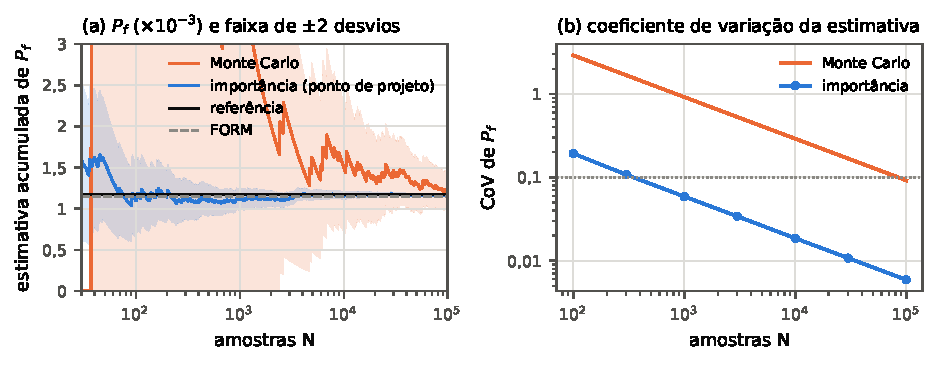
\includegraphics[width=\linewidth]{p1_convergencia}
\caption{Problema 1.
  (a) A estimativa acumulada de $P_f$, com a faixa de $\pm 2$ desvios: Monte Carlo e amostragem por importância.
  (b) O CoV da estimativa contra o número de amostras: a fórmula para Monte Carlo e a média de 20 rodadas para a
  amostragem por importância.}
\label{fig:p1}
\end{figure}

% =====================================================================================================
\section{Problema 2 (proposto): talude infinito não saturado sob chuva}
\label{sec:talude}

\subsection{Modelo}
O plano de ruptura é paralelo à superfície, à profundidade vertical $z$ (Figura~\ref{fig:talude}). Com a inclinação
$\beta_s$ e o peso específico $\gamma$, as tensões no plano são
\[
  \sigma_n = \gamma z \cos^2\beta_s, \qquad \tau = \gamma z \sin\beta_s \cos\beta_s .
\]
A chuva entra pela carga de pressão $h$ no plano: a pressão da água é $u_w = \gamma_w h$, com $h < 0$ sucção e $h > 0$
pressão positiva (lençol suspenso). Com a tensão efetiva de Bishop, $\sigma' = \sigma_n - \chi u_w$ e $u_a = 0$, o
fator de segurança é
\begin{equation}
  FS = \frac{c' + (\gamma z \cos^2\beta_s - \chi\, \gamma_w h) \tan\phi'}{\gamma z \sin\beta_s \cos\beta_s},
  \qquad g = FS - 1 .
  \label{eq:fs}
\end{equation}
Usei $\chi = 1$ ($\phi^b = \phi'$), como no material do \texttt{SlopeRandomField} (\texttt{p.chi = 1}). O código
também aceita $\chi = S_e(h)$ de van Genuchten, que é a tensão de sucção de Lu e Godt (2008), com a resistência por
sucção que satura.

\begin{figure}[H]
\centering
\begin{tikzpicture}[scale=0.85, >=Stealth]
  \fill[brown!12] (0,4) -- (5,-1) -- (5,-3) -- (0,2) -- cycle;
  \draw[thick] (0,4) -- (5,-1) node[right, font=\small] {superfície};
  \draw[thick, dashed, red!70!black] (0,2) -- (5,-3) node[right, font=\small] {plano de ruptura};
  \draw[fill=brown!35] (2,2) -- (2.6,1.4) -- (2.6,-0.6) -- (2,0) -- cycle;
  \draw[<->] (1.7,2) -- (1.7,0) node[midway, left, font=\small] {$z$};
  \draw (4,-2) -- (5.2,-2);
  \draw (4.7,-2) arc[start angle=0, end angle=-45, radius=0.7];
  \node[font=\small] at (5.05,-2.35) {$\beta_s$};
  \foreach \x in {0.6,1.4,2.2,3.0,3.8}
    \draw[->, blue!70!black] (\x, 4.9-\x) -- (\x, 4.15-\x);
  \node[blue!70!black, font=\small, anchor=west] at (2.2,3.1) {chuva};
  \draw[->, thick] (1.77,-0.83) node[below left, font=\small] {$\sigma_n$} -- (2.3,-0.3);
  \draw[->, thick] (2.3,-0.3) -- (1.77,0.23) node[left, font=\small] {$\tau$};
  \node[font=\small, align=left, anchor=west] at (5.3,1.0) {$h$: carga de pressão no plano\\
    \quad $h < 0$: sucção; $h > 0$: lençol suspenso\\[2pt]
    $c' \sim \mathrm{LN}(10\,\mathrm{kPa};\ 0{,}3)$\\ $\phi' \sim \mathrm{LN}(30^\circ;\ 0{,}1)$, $\rho(c', \phi') = -0{,}5$\\
    $h \sim \mathcal N(\mu_h;\ 0{,}5\,\mathrm{m})$};
\end{tikzpicture}
\caption{O talude infinito com o plano de ruptura à profundidade $z$ e as variáveis aleatórias.}
\label{fig:talude}
\end{figure}

\paragraph{Parâmetros.} Os do talude de Vargas Ceron et al.\ (2025), Tabela 2, e os do \texttt{SlopeMonteCarlo}:
\begin{itemize}
  \item geometria e solo: $\beta_s = 45^\circ$, $\gamma = 20$\,kN/m$^3$ e $\gamma_w = 9{,}81$\,kN/m$^3$, com $z = 2$\,m.
    Daí $\sigma_n = \tau = 20$\,kPa;
  \item variáveis aleatórias:
    \begin{itemize}
      \item $c' \sim \mathrm{LN}(10\,\mathrm{kPa};\ \cv\ 0{,}3)$;
      \item $\phi' \sim \mathrm{LN}(30^\circ;\ \cv\ 0{,}1)$;
      \item $h \sim \mathcal N(\mu_h;\ 0{,}5\,\mathrm{m})$;
    \end{itemize}
  \item correlação: $\rho(c', \phi') = -0{,}5$ nas variáveis físicas, o que dá $\rho_Z = $ \pDoisRhoZ{} pela
    Seção~\ref{sec:nataf}. O modelo de elementos finitos usa campos independentes, e os dois casos estão na
    Tabela~\ref{tab:erros2}.
\end{itemize}

\paragraph{A chuva.} A média $\mu_h$ é o cenário: $\mu_h = -2$\,m (sucção de cerca de 20\,kPa) antes da chuva, e
$\mu_h \to 0$ ou positivo depois. O desvio de $h$ resume, numa variável, a incerteza da resposta hidráulica, que no
modelo de elementos finitos vem do campo de $k_v$ (CoV de 60\,\%) e da própria chuva.

\paragraph{Referência.} Dados $\phi'$ e $h$, a falha é $c' < c'_{\mathrm{crit}} = \tau - (\sigma_n - \chi\gamma_w
h)\tan\phi'$, e $c'$ condicionada a $\phi'$ é lognormal. Então
\[
  P_f = \iint \varphi(z_2)\, f_h(h)\,
  \Phi\!\left(\frac{\ln c'_{\mathrm{crit}} - \lambda_c - \zeta_c \rho_Z z_2}{\zeta_c\sqrt{1 - \rho_Z^2}}\right)
  dz_2\, dh ,
\]
com o integrando nulo onde $c'_{\mathrm{crit}} \leq 0$. Essa integral 2D é calculada com quadratura adaptativa até
$P_f \sim 10^{-12}$.

\subsection{Dois cenários}
\label{sec:cenarios}

\begin{table}[H]
\centering\small
\caption{Problema 2: os cenários antes (A) e depois (B) da chuva. CoV para Monte Carlo e importância; erro de $P_f$
  para o FORM.}
\label{tab:cenarios}
\begin{tabular}{@{}l r r r r r r@{}}
\toprule
 & \multicolumn{3}{c}{Cenário A: $\mu_h = -2{,}0$\,m} & \multicolumn{3}{c@{}}{Cenário B: $\mu_h = -0{,}5$\,m} \\
\cmidrule(lr){2-4}\cmidrule(l){5-7}
Método & $N$ & $P_f$ & CoV ou erro & $N$ & $P_f$ & CoV ou erro \\
\midrule
Referência (integração) & --- & $1{,}535\times 10^{-4}$ & --- & --- & $0{,}1215$ & --- \\
FORM (HL-RF com Armijo) & 149 & $1{,}990\times 10^{-4}$ & $29{,}7\,\%$ & 49 & $0{,}1405$ & $15{,}7\,\%$ \\
Monte Carlo & $10^{3}$ & $0$ & --- & $10^{3}$ & $0{,}115$ & $8{,}8\,\%$ \\
Monte Carlo & $10^{6}$ & $1{,}45\times 10^{-4}$ & $8{,}3\,\%$ & $10^{6}$ & $0{,}121$ & $0{,}3\,\%$ \\
Importância (ponto de projeto) & $10^{3}$ & $1{,}512\times 10^{-4}$ & $7{,}0\,\%$ & $10^{3}$ & $0{,}1200$ & $4{,}3\,\%$ \\
Importância (ponto de projeto) & $10^{4}$ & $1{,}509\times 10^{-4}$ & $2{,}2\,\%$ & $10^{4}$ & $0{,}1208$ & $1{,}3\,\%$ \\
\midrule
$\beta$ do FORM & & $3{,}5414$ & & & $1{,}0781$ & \\
FS com as médias & & $1{,}644$ & & & $1{,}219$ & \\
$\alpha^2$ de $c'$, $\phi'$, $h$ & & \multicolumn{2}{l}{$0{,}13;\ 0{,}18;\ 0{,}69$} & & \multicolumn{2}{l@{}}{$0{,}23;\ 0{,}12;\ 0{,}65$} \\
Ponto de projeto $x^*$ & & \multicolumn{2}{l}{$6{,}60\,\mathrm{kPa};\ 28{,}0^\circ;\ -0{,}53\,\mathrm{m}$} & & \multicolumn{2}{l@{}}{$8{,}22\,\mathrm{kPa};\ 29{,}7^\circ;\ -0{,}07\,\mathrm{m}$} \\
\bottomrule
\end{tabular}

\end{table}

\begin{itemize}
  \item \textbf{Cenário B} (depois da chuva). $P_f = $ \pDoisBExato{}, da mesma ordem dos 11,5\,\% do talude do artigo
    (o talude infinito não é o mesmo talude, mas os parâmetros são). O FS com as médias é \pDoisBFS{}.
    \begin{itemize}
      \item Monte Carlo com $N = 1000$ basta: CoV de cerca de 9\,\%.
      \item O FORM superestima $P_f$ em \pDoisBErroForm{}.
    \end{itemize}
  \item \textbf{Cenário A} (antes da chuva). $P_f = $ \pDoisAExato{}, e o FS com as médias é \pDoisAFS{}.
    \begin{itemize}
      \item Monte Carlo com $N = 1000$ dá zero; com $10^6$ amostras, o CoV ainda é de 8\,\%.
      \item A amostragem por importância chega a um CoV de \pDoisACovIS{} com 1000 amostras.
      \item O FORM erra \pDoisAErroForm{}: o produto $(\sigma_n - \gamma_w h)\tan\phi'$ curva a superfície no espaço
        $U$ (Figura~\ref{fig:espacou}).
    \end{itemize}
  \item \textbf{Fatores de importância.} Nos dois cenários, a carga de pressão $h$ domina ($\alpha_h^2 \approx 0{,}65$
    a $0{,}69$), mais do que $c'$ e $\phi'$ juntos. No talude, a variável da chuva pesa mais que a resistência.
\end{itemize}

\begin{figure}[H]
\centering
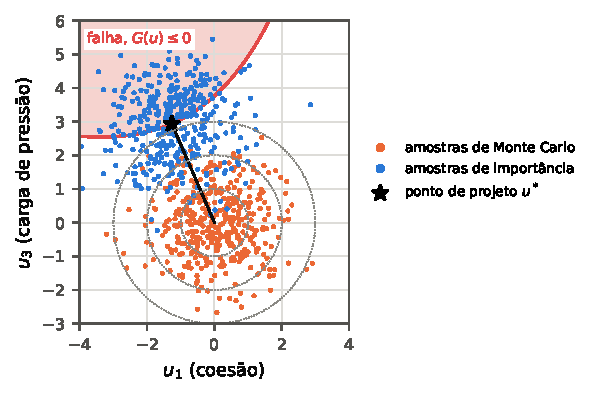
\includegraphics[width=0.78\linewidth]{p2_espaco_u}
\caption{Cenário A no plano $(u_1, u_3)$ (coesão e carga de pressão), com $u_2$ no valor do ponto de projeto: a
  superfície de falha e 400 amostras de cada método. Monte Carlo amostra em torno da origem, e quase nenhuma amostra
  falha. A amostragem por importância amostra em torno de $\bm u^*$, e cerca de metade das amostras falha.}
\label{fig:espacou}
\end{figure}

\subsection{O efeito dos erros do código original}
\label{sec:efeito}

Com o erro 1, o código usa $\bm z = L^{-1}\bm y$ na volta. A covariância implícita das $Z$ passa a ser $L^{-1}L^{-T}$,
e não $R_Z$. Com $\rho = -0{,}5$, a correlação implícita é $+$\pDoisRhoErro{} (o sinal se inverte), e o desvio de
$z_2$ é \pDoisDpErro{}. A Tabela~\ref{tab:erros2} mostra o efeito no FORM:
\begin{itemize}
  \item com o erro 1, $P_f$ fica \pDoisAErroL{} vezes maior no cenário A e \pDoisBErroL{} vez maior no B;
  \item sem a correção de Nataf (erro 6), a diferença é pequena, porque os CoV são pequenos;
  \item a correlação negativa entre $c'$ e $\phi'$ protege: com $\rho = 0$, o $P_f$ de referência fica 6 vezes maior
    no cenário A.
\end{itemize}

\begin{table}[H]
\centering\small
\caption{FORM com a transformação certa e com os erros do código original, e o caso independente.}
\label{tab:erros2}
\begin{tabular}{@{}l r r r r@{}}
\toprule
 & \multicolumn{2}{c}{Cenário A} & \multicolumn{2}{c@{}}{Cenário B} \\
\cmidrule(lr){2-3}\cmidrule(l){4-5}
Transformação usada no FORM & $\beta$ & $P_f$ do FORM & $\beta$ & $P_f$ do FORM \\
\midrule
correta (Nataf, $u = L^{-1} z$) & $3{,}5414$ & $1{,}99\times 10^{-4}$ & $1{,}0781$ & $0{,}140$ \\
com o erro do \texttt{FromXtoY} ($L$ no lugar de $L^{-1}$) & $2{,}5112$ & $6{,}02\times 10^{-3}$ & $0{,}8076$ & $0{,}210$ \\
sem a correção de Nataf ($R_Z = R_X$) & $3{,}5239$ & $2{,}13\times 10^{-4}$ & $1{,}0733$ & $0{,}142$ \\
\midrule
$c'$ e $\phi'$ independentes ($\rho = 0$), FORM & $3{,}0658$ & $1{,}09\times 10^{-3}$ & $0{,}9468$ & $0{,}172$ \\
$c'$ e $\phi'$ independentes, referência & $3{,}1067$ & $9{,}46\times 10^{-4}$ & $0{,}9995$ & $0{,}159$ \\
\bottomrule
\end{tabular}

\end{table}

\subsection{HL-RF com e sem a busca de Armijo}
\label{sec:armijo}

O HL-RF puro oscila em torno do ponto de projeto e não converge para $\mu_h \leq$ \pDoisNaoConvMax{}\,m. Ali, depois
de 100 iterações, o $\beta$ está errado em até 30\,\% (Tabela~\ref{tab:hlrf}). Com a busca de Armijo, ele converge em
9 a 21 iterações nesses cenários. Num modelo de elementos finitos, cada iteração do HL-RF puro que não converge custa $2n + 1$
análises.

\begin{table}[H]
\centering\small
\caption{O HL-RF puro e com a busca de Armijo ao longo dos cenários de chuva.}
\label{tab:hlrf}
\begin{tabular}{@{}r r r r r r r@{}}
\toprule
$\mu_h$ (m) & FS médio & $P_f$ (referência) & $\beta$ (HL-RF com Armijo) & iterações & $\beta$ (HL-RF puro) & iterações \\
\midrule
$-4{,}00$ & $2{,}210$ & $2{,}86\times 10^{-12}$ & $6{,}8361$ & 21 & $4{,}8949$ & não converge (100) \\
$-3{,}50$ & $2{,}069$ & $6{,}25\times 10^{-10}$ & $6{,}0200$ & 15 & $4{,}7444$ & não converge (100) \\
$-3{,}00$ & $1{,}927$ & $7{,}39\times 10^{-8}$ & $5{,}1975$ & 12 & $4{,}5865$ & não converge (100) \\
$-2{,}50$ & $1{,}785$ & $4{,}65\times 10^{-6}$ & $4{,}3705$ & 9 & $4{,}3699$ & não converge (100) \\
$-2{,}00$ & $1{,}644$ & $1{,}53\times 10^{-4}$ & $3{,}5414$ & 21 & $3{,}5414$ & 35 \\
$-1{,}00$ & $1{,}361$ & $0{,}0243$ & $1{,}8900$ & 11 & $1{,}8900$ & 11 \\
$0{,}00$ & $1{,}077$ & $0{,}350$ & $0{,}2877$ & 4 & $0{,}2877$ & 4 \\
$0{,}50$ & $0{,}936$ & $0{,}642$ & $-0{,}4639$ & 5 & $-0{,}4639$ & 5 \\
\bottomrule
\end{tabular}

\end{table}

\subsection{Curva de fragilidade}
\label{sec:fragilidade}

A Figura~\ref{fig:fragilidade} mostra $P_f(\mu_h)$, de $3 \times 10^{-12}$ ($\mu_h = -4$\,m) a 0,64 ($\mu_h = 0{,}5$\,m):
\begin{itemize}
  \item o FORM superestima $P_f$ em 6\,\% ($\mu_h = 0{,}5$\,m) a 42\,\% ($\mu_h = -4$\,m). O erro cresce nos
    cenários secos, em que $\beta$ é maior e a curvatura da superfície pesa mais;
  \item a amostragem por importância com 1000 amostras fica a até 2 desvios da referência em todos os níveis, com CoV
    de 3 a 10\,\%. Isso exige um bom ponto de projeto, e o do FORM com Armijo é bom;
  \item Monte Carlo com 1000 amostras só vê $P_f \gtrsim 10^{-2}$;
  \item a importância de $c'$ cresce quando a sucção acaba ($\mu_h \to 0$).
\end{itemize}

\begin{figure}[H]
\centering
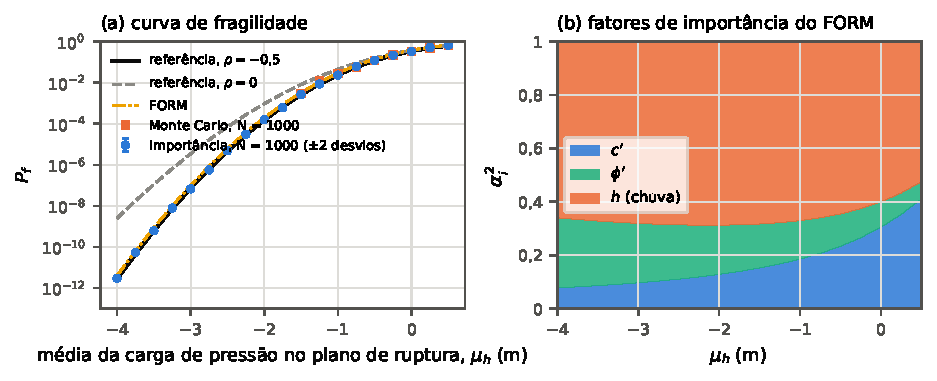
\includegraphics[width=\linewidth]{p2_fragilidade}
\caption{Problema 2. (a) A curva de fragilidade $P_f(\mu_h)$: referência com $\rho = -0{,}5$ e com $\rho = 0$, FORM,
  importância e Monte Carlo com 1000 amostras. (b) Os fatores de importância do FORM.}
\label{fig:fragilidade}
\end{figure}

% =====================================================================================================
\section{Uso no talude com chuva e campos aleatórios}
\label{sec:aplicacao}

\subsection{A correspondência}
No \texttt{SlopeMonteCarlo} (e no \texttt{SlopeRandomField}), cada realização tira os coeficientes $\xi_k$ da expansão
de Karhunen-Loève dos três campos ($c'$, $\phi'$ e $k_v$; \texttt{RandomFields::Sample}). Cada campo é
$c'(\bm x) = \exp(\lambda + \zeta Z(\bm x))$, com $Z = \sum_k \sqrt{\lambda_k} \xi_k f_k(\bm x)$. O fator $\Gamma$ vem
do GIM. A correspondência com as seções anteriores:

\begin{table}[H]
\centering\small
\caption{O talude infinito e o talude de elementos finitos.}
\label{tab:corresp}
\begin{tabular}{@{}p{4.2cm} p{5.0cm} p{6.6cm}@{}}
\toprule
& Problema 2 & Talude com campos aleatórios \\
\midrule
Espaço $\bm U$ & $(u_c, u_\phi, u_h)$, $n = 3$ & os $\xi_k$ dos três campos: $n = 3M = 6000$ com $M = 2000$. Já são
  normais padrão independentes: não há transformação de Nataf a fazer \\
Marginais & lognormal e normal & lognormal ponto a ponto (\texttt{klsep::Lognormal}), exata \\
Correlação $c'$--$\phi'$ & $\rho_Z$ e Cholesky & os campos são independentes. Com correlação cruzada, mesmo núcleo:
  $(\xi_{c,k}, \xi_{\phi,k}) = L_2(\eta_{1,k}, \eta_{2,k})$ em cada modo, com $L_2$ o Cholesky de
  $[\,1\ \rho_Z;\ \rho_Z\ 1\,]$ (o \texttt{ComputeJYZ} corrigido, modo a modo) \\
$G(\bm u)$ & $FS - 1$, Eq.~\eqref{eq:fs} & $\Gamma(\bm\xi) - 1$: uma análise (percolação, GIM e refinamento) \\
Chuva & $\mu_h$ & a intensidade e a duração do transiente; $P_f(t)$ ou $P_f$ por cenário \\
Custo de $G$ & microssegundos & cerca de 95\,s por realização no fermi, com 4 níveis
  (\path{SlopeMonteCarlo/cluster/README.md}) \\
\bottomrule
\end{tabular}
\end{table}

\subsection{Qual método e quando}
\begin{itemize}
  \item \textbf{$P_f \gtrsim 5\,\%$} (a configuração de referência do artigo: 11,5\,\%; o nosso estudo de refinamento:
    10,8\,\%). Monte Carlo basta:
    \begin{itemize}
      \item $N = 1000$ dá CoV de 9\,\%, e $N = 10\,000$, cerca de 3\,\%;
      \item a amostragem por importância reduziria $N$ de 2 a 4 vezes (no cenário B, \pDoisBNisDez{} contra
        \pDoisBNmcDez{} realizações para um CoV de 10\,\%), mas exige achar o deslocamento.
    \end{itemize}
  \item \textbf{$P_f \lesssim 10^{-2}$}: outros cenários, como menos chuva, um talude menos íngreme ou um solo mais
    resistente; probabilidades de projeto ($\beta \approx 2{,}5$ a $3$); e o começo da curva $P_f(t)$.
    \begin{itemize}
      \item Monte Carlo para um CoV de 10\,\% precisa de $N \approx 100/P_f$ realizações: $10^5$ análises para
        $P_f = 10^{-3}$, cerca de 2600\,h de processo no fermi.
      \item A amostragem por importância precisa de algumas centenas: no cenário A, \pDoisANisDez{} contra
        \pDoisANmcDez{}.
    \end{itemize}
  \item \textbf{FORM direto no modelo de elementos finitos: não.}
    \begin{itemize}
      \item O gradiente por diferenças custa $2n$ análises por iteração (centrais) ou $n + 1$ (progressivas). Com
        $n = 6000$ e diferenças progressivas, são cerca de $6000 \times 95\,\mathrm{s} \approx 6{,}6$ dias de
        processo por iteração.
      \item O $\Gamma$ do GIM tem a tolerância do próprio método. O passo das diferenças teria de ser grande (por
        exemplo, $0{,}1$ a $0{,}3$ em $u$), ou o gradiente sai ruído.
      \item O FORM só é viável com poucos modos ($M = 20$ a 50 por campo, $n \leq 150$): cerca de 4\,h por iteração
        num processo, ou minutos com as análises em paralelo. Serve para os fatores de importância (quais campos e
        quais modos pesam) e como ponto de partida da amostragem por importância.
    \end{itemize}
\end{itemize}

\subsection{Amostragem por importância sem gradiente: o caminho proposto}
\label{sec:proposta}

O deslocamento ótimo de uma normal com covariância identidade, no sentido da entropia cruzada (Rubinstein e Kroese,
2004), é a média condicional à falha: $\bm u^\dagger = \E[\bm U \mid G(\bm U) \leq 0]$. Ela pode ser estimada com as
realizações que já existem:
\begin{enumerate}
  \item \textbf{Piloto.} Use as realizações de Monte Carlo já feitas. Os $\bm\xi$ de cada uma são reprodutíveis pela
    semente (\texttt{klsep::Normal(semente $\cdot$ 0x9E37... + 3 real + campo)}).
  \item \textbf{Deslocamento.} Calcule a média dos $\bm\xi$ das realizações com $\Gamma < 1$. Se forem poucas,
    use as 10\,\% com menor $\Gamma$, como um nível intermediário da entropia cruzada: o GIM dá $\Gamma$ contínuo, e os
    níveis $\Gamma \leq \gamma_1$, com $\gamma_1 > \gamma_2 > \cdots > 1$, saem de graça.
  \item \textbf{Regularização.} Mantenha o deslocamento só nos $K$ primeiros modos de cada campo (os de maior
    $\lambda_k$; $K = 20$ a 50) e zere os outros. Cada componente da média tem ruído de cerca de $1/\sqrt{N_f}$. Com
    $n = 6000$ componentes, $\|\bm\delta\|^2 \approx n/N_f$, e o $\E[w^2]$ cresceria como $e^{\|\bm\delta\|^2}$
    (Seção~\ref{sec:is}).
  \item \textbf{Amostragem.} Rode $N_{\mathrm{IS}}$ realizações com $\bm\xi = \bm u^\dagger + \bm\varepsilon$. Grave
    $\Gamma$ e $\ln w = -\bm\xi\cdot\bm u^\dagger + \frac12\|\bm u^\dagger\|^2$. Daí
    $\hat P_f = \frac1N\sum I[\Gamma < 1]\,w$, e o CoV vem da amostra.
  \item \textbf{Iteração.} Se o piloto não tiver falhas, repita os passos 2 a 4 com níveis de $\Gamma$ cada vez mais
    baixos (entropia cruzada em vários níveis), ou use a simulação por subconjuntos (Au e Beck, 2001). Ela não precisa
    de deslocamento: cerca de $N$ análises por nível e $\log_{10}(1/P_f)$ níveis.
\end{enumerate}

\paragraph{A mudança no código.} Ela é pequena e fica em \texttt{RandomFields::Sample}, no arquivo
\path{Projects/Common/SlopeFields.cpp}:
\begin{itemize}
  \item depois de sortear \texttt{fXi}, some o deslocamento, lido de um arquivo (por exemplo, \texttt{DESLOCAMENTO}
    com 3 colunas e $M$ linhas);
  \item devolva $\ln w$ e grave-o no CSV da realização, ao lado de $\Gamma$;
  \item a estatística do \texttt{SlopeMonteCarlo} passa a usar $\sum I w/N$ em vez de $n_f/N$.
\end{itemize}

\paragraph{Uma vantagem para a chuva.} Os pesos não dependem do instante. Com $\Gamma$ calculado em vários instantes do
transiente, uma única amostragem dá $P_f(t)$ em todos eles. Ela é mais eficiente perto do instante para o qual o
deslocamento foi escolhido.

\paragraph{O talude infinito como teste.} O problema 2 serve para ensaiar a amostragem antes de gastar análises: um
modelo barato com os mesmos parâmetros, que dá a ordem de grandeza de $P_f$ por cenário e mostra quais variáveis pesam
(lá, a carga de pressão). O ajuste lognormal de $\Gamma$ do \texttt{SlopeMonteCarlo} extrapola $P_f$ de graça, mas
depende do modelo de distribuição. A amostragem por importância não tem viés.

% =====================================================================================================
\section{Conclusões}
\begin{itemize}
  \item O FORM do código original estava certo ($\beta = 3{,}049$), mas a transformação $x \leftrightarrow y$ tinha
    $L$ e $L^{-1}$ trocados e a volta errada. Com correlação, isso muda $P_f$ por um fator de até 30 no problema
    proposto.
  \item O código revisado separa o modelo probabilístico (Nataf), a função de estado limite (escrita uma vez, nas
    variáveis físicas) e os métodos (FORM com Armijo, Monte Carlo e importância, com o CoV).
  \item Com $P_f \sim 10^{-3}$, Monte Carlo com 1000 amostras não serve. A amostragem por importância no ponto de
    projeto dá CoV de 6\,\% com as mesmas 1000.
  \item No talude infinito sob chuva, a carga de pressão domina $P_f$. O FORM superestima $P_f$ em 6 a 42\,\%, e o HL-RF
    sem a busca de Armijo não converge nos cenários secos.
  \item No talude de elementos finitos, com $P_f \approx 11\,\%$, Monte Carlo basta. Para $P_f$ pequenos, o caminho é
    a amostragem por importância com o deslocamento estimado das realizações que falham, restrito aos primeiros modos,
    ou a simulação por subconjuntos. O FORM direto não é viável com 6000 variáveis.
\end{itemize}

% =====================================================================================================
\begin{thebibliography}{99}
\bibitem{au2001} Au, S.-K.; Beck, J. L. (2001). Estimation of small failure probabilities in high dimensions by subset
  simulation. \emph{Probabilistic Engineering Mechanics} 16(4), 263--277.
\bibitem{au2003} Au, S.-K.; Beck, J. L. (2003). Importance sampling in high dimensions. \emph{Structural Safety} 25(2),
  139--163.
\bibitem{hasofer} Hasofer, A. M.; Lind, N. C. (1974). Exact and invariant second-moment code format. \emph{Journal of
  the Engineering Mechanics Division} (ASCE) 100(1), 111--121.
\bibitem{liu} Liu, P.-L.; Der Kiureghian, A. (1986). Multivariate distribution models with prescribed marginals and
  covariances. \emph{Probabilistic Engineering Mechanics} 1(2), 105--112.
\bibitem{lu} Lu, N.; Godt, J. (2008). Infinite slope stability under steady unsaturated seepage conditions.
  \emph{Water Resources Research} 44, W11404.
\bibitem{melchers} Melchers, R. E.; Beck, A. T. (2018). \emph{Structural Reliability Analysis and Prediction}, 3.\ ed.
  Wiley.
\bibitem{rackwitz} Rackwitz, R.; Fiessler, B. (1978). Structural reliability under combined random load sequences.
  \emph{Computers \& Structures} 9(5), 489--494.
\bibitem{rubinstein} Rubinstein, R. Y.; Kroese, D. P. (2004). \emph{The Cross-Entropy Method}. Springer.
\bibitem{ceron} Vargas Ceron, Cecílio, Linn e Maghous (2025). O artigo de referência do \texttt{SlopeRandomField} e do
  \texttt{SlopeMonteCarlo} (Seção 6 e Tabela 2).
\bibitem{zhang} Zhang, Y.; Der Kiureghian, A. (1995). Two improved algorithms for reliability analysis. Em: Rackwitz,
  R.; Augusti, G.; Borri, A. (eds.), \emph{Reliability and Optimization of Structural Systems}. Springer.
\end{thebibliography}

% =====================================================================================================
\appendix
\section{Como reproduzir}
\begin{itemize}
  \item \textbf{Mathematica:} abra \texttt{confiabilidade.wl} e use \emph{Run All Code}. Os valores esperados estão nos
    comentários. As estimativas de Monte Carlo e de importância mudam com a semente, dentro do CoV impresso.
  \item \textbf{Python:} em \path{python/}, \texttt{python3 problemas.py} (cerca de 2\,min) grava
    \path{doc/tabelas}, \path{doc/figuras} e \path{dados/p2_fragilidade.csv}. Depois, em \path{doc/},
    \texttt{latexmk -pdf confiabilidade.tex}.
\end{itemize}

\section{O código revisado}
\lstinputlisting{../confiabilidade.wl}

\end{document}
